\chapter{A Modular View of Parsing}
\label{cha:ParserOverview}

Last time we saw that Marr's three levels of analysis are a useful guideline with respect to how one might think about the distinction between grammar and parser in linguistics.
We also extended this idea --- that one and the same device can be described at distinct levels of abstraction --- to the parser itself. We may thus differentiate between an idealized competence parser --- the full specification of the human parser --- and the performance parser, i.e.\ how the parser actually behaves when executed by the neural hardware of the human brain.
But even if we disregard cognition for a moment and think about parsing in purely computational terms, it quickly becomes evident that there's many different ways of defining a parser, some more specific than others.
In computer science, this is mostly a matter of convenience and generality, where abstraction pays off when studying the mathematics of parsing whereas the actual implementation in some programming language requires a lot more detail.

For this course, on the other hand, abstraction is a matter of explanation: eventually, we want to relate parsing techniques to human sentence processing.
If our description of the parser abstracts away from, say, how intermediate information is stored and retrieved, we're making the empirical assumption that these aspects of the parser are irrelevant for the psycholinguistic phenomena we observe.
So before we even start any kind of empirically minded work, we have to get a better understanding of the different levels of abstraction, and in particular, what exactly we are abstracting away from.


\section{The Most General View of Parsing}
\label{sec:ParserOverview_MostGeneralView}

One of the cornerstones of transformational grammar is the inverted T-model, a metaphor for the place of syntax in the language faculty.
%
\begin{center}
    \begin{tikzpicture}
        \node (root) at (0,0) {lexicon};
        \node (spell-out) at (0,-4em) {spell-out};
        \node (PF) [below left=of spell-out] {PF\slash pronunciation};
        \node (LF) [below right=of spell-out] {LF\slash interpretation};

        \draw (root) to (spell-out);
        \draw[decorate,decoration={snake,post length=.75em},->] (spell-out) to node [above, near end] {\Large \PFmapping} (PF);
        \draw[decorate,decoration={snake,post length=.75em},->] (spell-out) to node [above, near end] {\Large \LFmapping} (LF);
    \end{tikzpicture}
\end{center}
%
The canonical interpretation of this diagram is procedural in nature:
%
\begin{enumerate}
    \item syntax builds structures from the items in the lexicon (or the numeration in earlier versions of Minimalist syntax),
    \item at some point spell-out takes place and creates two copies of the built tree \citep[229]{Chomsky95b},
    \item one copy is turned into a pronounceable structure by a variety of processes summarily referred to as $\PFmapping$,
    \item the other copy is turned into an interpretable structure by processes jointly referred to as $\LFmapping$.
\end{enumerate}
%
There is, however, a more parsimonious interpretation of this model:
%
\begin{itemize}
    \item the grammar specifies a set of well-formed representations (e.g.\ phrase structure trees),
    \item we can define various functions for mapping these representations to other structures; in the case at hand, a function $\PFmapping$ from trees to strings and a function $\LFmapping$ from trees to semantic interpretations
\end{itemize}

Notice that this more agnostic perspective generalizes the T-model from natural language to all kinds of rule-based systems.
Just consider programming: a program is a highly structured object that has a linear realization in the form of its source code (its image under $\PFmapping$) and a realization in terms of the instructions carried out by the computer it is run on (its image under $\LFmapping$).
Why does this matter? Because it gives us the most general and abstract description of a parser.
%
\begin{description}
    \item[Parsing as inverted pronunciation] Given a grammar $G$ with mapping $\PFmapping$ from trees to strings, a parser for $G$ is a device that computes $\inverse{\PFmapping}$ (the inverse of $\PFmapping$).
\end{description}

\begin{examplebox}[The $\inverse{\PFmapping}$ parser]
    Suppose that our grammar has exactly two trees $s$ and $t$ whose string yield is \emph{Time flies like an arrow}.
    %
    \begin{center}
        \begin{tikzpicture}
            \Tree
                [.S
                    [.NP
                        [.N time ]
                    ]
                    [.VP
                        [.V flies ]
                        [.PP
                            [.P like ]
                            [.NP
                                [.Art an ]
                                [.N arrow ]
                            ]
                        ]
                    ]
                ]
        \end{tikzpicture}
        %
        \hspace{2em}
        %
        \begin{tikzpicture}
            \Tree
                [.S
                    [.NP
                        [.N
                            [.N time ]
                            [.N flies ]
                        ]
                    ]
                    [.VP
                        [.V like ]
                        [.NP
                            [.Art an ]
                            [.N arrow ]
                        ]
                    ]
                ]
        \end{tikzpicture}
    \end{center}
    %
    Like any other function, $\PFmapping$ can be viewed as a set of pairs $\tuple{a,b}$, which means that $a$ is mapped to $b$ by $\PFmapping$.
    So for our example, $\PFmapping$ is some set that contains at least $\tuple{s,\text{time flies like an arrow}}$ and $\tuple{t,\text{time flies like an arrow}}$.
    The inverse of $\PFmapping$ is simply the set that contains the pair $\tuple{b,a}$ iff $\tuple{a,b}$ is a member of $\PFmapping$.
    Hence $\inverse{\PFmapping}$ contains both $\tuple{\text{time flies like an arrow},s}$ and $\tuple{\text{time flies like an arrow},t}$.
    Given our interpretation of these pairs, this just means that this string can be mapped to $s$ and $t$.
    And from this it follows that any device that correctly computes $\inverse{\PFmapping}$ picks out $s$ and $t$ as the only licit trees for \emph{time flies like an arrow} --- which is exactly what we want a parser to do.
\end{examplebox}

\begin{exercise}
    If $\inverse{\PFmapping}$ is parsing, what is $\inverse{\LFmapping}$?
\end{exercise}


\section{One Step Down: Parsing as Grammar Intersection}
\label{sec:ParserOverview_IntersectionParsing}

\subsection{Parsing as Generation}
The obvious problem with the previous view of parsing is that it tells us nothing about how the actual process is accomplished: if we don't know how to compute $\inverse{\PFmapping}$, there is little we can do.
Now for some choices of $\PFmapping$ there are some very general algorithms for computing $\inverse{\PFmapping}$ (for example if $\PFmapping$ can be defined in terms of monadic second-order logic, the extension of first-order logic with quantification over sets).
But for the purpose of relating parsing to human sentence processing, this perspective is still too general.
It can provide profound insights into the overall computational difficulty of the parsing problem, but it is too coarse to have any bearing on specific processing phenomena or assumptions about the human parser.

A slightly more concrete view is offered by \emph{intersection parsing}.
Intersection parsing builds on the insight that all common grammar formalisms are closed under intersection with finite languages.%
\footnote{
    The closure property actually extends to all regular string languages, which includes all finite languages.
}
That is to say, if $G$ is a grammar of formalism $\mathcal{F}$, and one takes the intersection of the language $L$ generated by $G$ and some arbitrary finite language $L_F$, then this language $L(G) \cap L_F$ can be generated by some grammar $G'$ belonging to formalism $\mathcal{F}$.
Crucially, the proofs for this theorem are constructive in nature, which means that they actually provide a procedure for constructing $G'$ from $G$ and $L_F$.

This opens up the following strategy:
%
\begin{enumerate}
    \item Suppose $i$ is our input sentence that needs to be parsed with respect to grammar $G$.
        Let $L \is \setof{i}$ be the language whose only well-formed string is $i$.
    \item Construct the grammar $G'$ that generates $L(G) \cap L$.
    \item Use $G'$ to infer the valid trees for $i$.
\end{enumerate}
%
But how exactly does one handle the third step?
Isn't that exactly the parsing problem we started out with, except that we're now operating with a different grammar?

As so often, the answer is both yes and no.
First, let's make two assumptions about our initial grammar $G$.
%
\begin{description}
    \item[No loops] The grammar does not generate any trees with a sequence of unary branches where some non-terminal symbol occurs more than once.
    \item[No empty heads] The empty string $\emptystring$ is not a valid terminal symbol.
\end{description}
%
\begin{examplebox}[A tree with two loops]
    The tree below contains two loops.
    %
    \begin{center}
        \begin{tikzpicture}
            \Tree
                [.S
                    [.T
                        [.S
                            [.NP
                                [.N John ]
                            ]
                            [.VP
                                [.T
                                    [.S
                                        [.VP
                                            [.V punched ]
                                            [.NP
                                                [.N Mary ]
                                            ]
                                        ]
                                    ]
                                ]
                            ]
                        ]
                    ]
                ]
        \end{tikzpicture}
    \end{center}
\end{examplebox}
%
One can prove that this two assumptions jointly imply the property below.
%
\begin{description}
    \item[Bounded tree size] A grammar $G$ has the \emph{bounded tree size property} iff it holds for every sentence $s$ generated by $G$ that the size of each tree that $G$ assigns to $s$ is finitely bounded by the length of $s$.
\end{description}
%
The intuitive reasoning is as follows:
In order to increase the size of a tree, one has to apply a rewrite rule.
Every rewrite rule increases the number of symbols that are expanded into one or more symbols.
If we can't have loops, that puts an upper bound on the length of unary branches.
If we can't have empty heads, then every symbol that is rewritten by at least two symbols will eventually bring about the addition of at least two terminal symbols to the generated string.
So the length of the string limits how many rewrite rules can be applied, which in turn limits the size of the trees that can be assigned to the string.

The bounded tree size property, in turn, guarantees that $G'$ in step 3 above assigns only finitely many trees to the input sentence.
%
\begin{lemma}
    If grammar $G$ has the bounded tree size property, it assigns only finitely many trees to every string in the language it generates.
\end{lemma}
%
This result may seem obvious, but it is the very reason why it is dead easy to use $G'$ to infer the valid trees for $i$: the only trees well-formed with respect to $G'$ are those that $G$ assigns to $i$.
That is to say, in order to determine the licit trees for $i$ we just have list the trees generated by $G'$.
And since the latter by assumption has the bounded tree size property, there's only finitely many trees that $G'$ generates.
We can find them all by simply applying all the rewrite rules of $G'$ in all possible ways (this step will finish after a finite amount of time since there's only a finite number of trees that need to be generated).

\begin{description}
    \item[Intersection parsing] Suppose $i$ is our input sentence that needs to be parsed with respect to grammar $G$.
        Let $L \is \setof{i}$ be the language whose only well-formed string is $i$.
        %
        \begin{itemize}
            \item Construct the grammar $G'$ that generates $L(G) \cap L$.
            \item Apply all rewrite rules of $G'$ in all possible ways to obtain the set of trees generated by $G'$.
                This is also the set of trees that $G$ assigns to $i$.
        \end{itemize}
\end{description}

\begin{exercise}
    As linguists we are very fond of our empty heads, so the requirement that the empty string may not appear on the right hand side of any rule seems overly strong.
    Can you think of a relaxed version of the ban against empty heads that is compatible with linguistic practice but also preserves the bounded tree size property?
\end{exercise}
%
\begin{exercise}
    Would the procedure above also work for grammars that do not enjoy the bounded tree size property?
    What exactly would we lose?
\end{exercise}

\subsection{Constructing the Intersection Grammar}

For CFGs the intersection grammar can be constructed very easily using a technique due to \citet{BarHillel.etal61}.
Essentially, we subscript each terminal with the start and end position of the substring it covers in the input sentence.
That way, we end up with a grammar where each non-terminal can only generate a specific string that corresponds to a continuous part of the input sentence --- each symbol is now tied to specific positions in the string.

Suppose we have the following CFG.
%
\begin{center}
    \begin{tabular}{rcl@{\hspace{5em}}rcl}
        S  & \rewrite & NP VP &  N & \rewrite & John\\
        NP & \rewrite & N     &  N & \rewrite & Mary \\
        VP & \rewrite & V NP  &  V & \rewrite & punched\\
    \end{tabular}
\end{center}
%
This grammar generates four sentences.
%
\begin{exe}
    \ex
    \begin{xlist}
        \ex John punched John.
        \ex John punched Mary.
        \ex Mary punched John.
        \ex Mary punched Mary.
    \end{xlist}
\end{exe}
%
We will now construct an intersection grammar that generates all parses for the sentence \emph{John punched Mary}.
Integers are used to refer to specific positions in the input string as illustrated below.
%
\begin{center}
    \begin{tikzpicture}
        \foreach \Position in {0,1,2,3}
            \node[draw,circle] (\Position) at ($\Position*(6em,0)$) {\Position};

        \foreach \Word/\Start/\End in { John/0/1,
                                        punched/1/2,
                                        Mary/2/3%
                                      }
            \draw[->] (\Start) to node [above] {\Word} (\End);
    \end{tikzpicture}
\end{center}

We could construct the intersection grammar bottom-up, starting with the rules generating leaves, but we will proceed top-down instead.
So consider the rule S \rewrite\ NP VP\@.
Since S is the root of the generated tree, it must span the whole input string.
Consequently, we replace S by $_0$S$_3$.
It is also obvious that the NP starts at position $0$ and the VP ends at position $3$.
So the new rewrite rule must be $_0$S$_3$ \rewrite\ $_0$NP$_i$ $_i$VP$_3$, where $i$ is some integer between $0$ and $3$.
A computer would try all possible options and then discard the ones that never occur in any tree for the input sentence, but we can inspect the original grammar and see immediately that its NPs only generate strings containing exactly one word.
Therefore the NP must span from $0$ to $1$ and we have $_0$S$_3$ \rewrite\ $_0$NP$_1$ $_1$VP$_3$.
Continuing in this fashion with the other rewrite rules, we eventually obtain the intersection grammar.
%
\begin{center}
    \begin{tabular}{rcl@{\hspace{5em}}rcl}
        $_0$S$_3$  & \rewrite & $_0$NP$_1$ $_1$VP$_3$
        \\
        $_0$NP$_1$ & \rewrite & $_0$N$_1$
                   & 
        $_0$N$_1$  & \rewrite & John
        \\
        $_2$NP$_3$ & \rewrite & $_2$N$_3$
                   & 
        $_2$N$_3$  & \rewrite & Mary
        \\
        $_1$VP$_3$ & \rewrite & $_1$V$_2$ $_2$NP$_3$
                   & 
        $_1$V$_2$  & \rewrite & punched
    \end{tabular}
\end{center}

Note that we now have multiple NP rules that are almost identical except for their indices, which is expected because we have multiple NPs covering different spans of the input.
This grammar also generates only one tree, which is shown below.
%
\begin{center}
    \begin{tikzpicture}
        \Tree
            [.$_0$S$_3$
                [.$_0$NP$_1$
                    [.$_0$N$_1$
                        John
                    ]
                ]
                [.$_1$VP$_3$
                    [.$_1$V$_2$
                        punched
                    ]
                    [.$_2$NP$_3$
                        [.$_2$N$_3$
                            Mary
                        ]
                    ]
                ]
            ]
    \end{tikzpicture}
\end{center}
%
In principle it might be possible for an intersection grammar to generate an infinite number of trees (as a single input may have an infinite number of possible analyses).
In that case it obviously isn't practical to generate all trees, but we do not need to.
The intersection grammar fully represents the set of possible parses, just like the original grammar fully represents the set of well-formed trees of the language.
So whatever you want to do with the parse trees, you can lift it to an operation over the intersection grammar and get your desired result this way.
For this reason, intersection grammars are also called \emph{parse forests}.

While intersection parsing is very elegant, it still abstracts away from too many issues that are relevant to us.
In particular, the \emph{incrementality of parsing} no longer plays a role.
Syntactic processing operates in an incremental fashion;
the parser doesn't wait for the entire sentence to be uttered before it starts working, it kicks off as soon as the first word has been heard.
The parsing as intersection approach, on the other hand, needs to know the entire input sentence in order to construct the grammar that will be used for inferring the tree structures.
Since pretty much all interesting phenomena in syntactic processing are related to incrementality in some form or another, intersection parsing is also too coarse for our purposes.
We have to get closer to the algorithmic level of description.
But try to keep intersection parsing in the back of your head --- in the next weeks, you will (hopefully) come to realize that parsers are essentially algorithms for generating intersection grammars on the fly.


\section{Towards the Algorithmic Level}
\label{sec:ParserOverview_AlgorithmicLevel}

\subsection{The Three Modules of a Parser}
\label{sub:ParserOverview_Modules}

Modern parsing theory treats parsers as the combination of three distinct modules.
%
\begin{description}
    \item[Parsing schema]
        A rule system that specifies
        \begin{itemize}
            \item the general form of \emph{parsing items},
            \item the possible initial items,
            \item the desired final items,
            \item a finite number of \emph{inference rules} for constructing new items from old ones
        \end{itemize}
        %
    \item[Control structure]
        A system for choosing
        \begin{itemize}
            \item which inference rules to apply at any given point during the parse, and
            \item in which order they should be applied.
        \end{itemize}
        %
    \item[Data structure]
        A system for storing and retrieving parsing items.
\end{description}
%
\begin{examplebox}[A naive parser for CFGs]
    Suppose we want to parse the sentence \emph{John punched Mary} with the same CFG as before, which is repeated here for your convenience.
    %
    \begin{center}
        \begin{tabular}{rcl@{\hspace{5em}}rcl}
            S  & \rewrite & NP VP &  N & \rewrite & John\\
            NP & \rewrite & N     &  N & \rewrite & Mary \\
            VP & \rewrite & V NP  &  V & \rewrite & punched\\
        \end{tabular}
    \end{center}
    %
    Obviously there is only one valid tree for this sentence.
    %
    \begin{center}
        \begin{tikzpicture}
            \Tree
                [.S
                    [.NP
                        [.N John ]
                    ]
                    [.VP
                        [.V punched ]
                        [.NP
                            [.N Mary ]
                        ]
                    ]
                ]
        \end{tikzpicture}
    \end{center}
    %
    But how do we get this tree?
    In your syntax class, you might have learned to draw a table like the one below.
    %
    \begin{center}
        \begin{tabular}{r|l}
            \textbf{item}     & \textbf{rule}\\
            S                 & start symbol\\
            NP VP             & S \rewrite\ NP VP\\
            N VP              & NP \rewrite\ N\\
            John VP           & N \rewrite\ John\\
            John V NP         & VP \rewrite\ V NP\\
            John punched NP   & V \rewrite\ punched\\
            John punched N    & NP \rewrite\ N\\
            John punched Mary & N \rewrite\ Mary
        \end{tabular}
    \end{center}
    %
    What we have done is to identify an initial item, S, followed by a list of the rules that we used to rewrite items.
    Note that the order we applied the rules in is mostly irrelevant.
    %
    \begin{center}
        \begin{tabular}{r|l}
            \textbf{item}     & \textbf{rule}\\
            S                 & start symbol\\
            NP VP             & S \rewrite\ NP VP\\
            NP V NP           & VP \rewrite\ V NP\\
            N V NP            & NP \rewrite\ N\\
            N V N             & NP \rewrite\ N\\
            John V N          & N \rewrite\ John\\
            John V Mary       & N \rewrite\ Mary\\
            John punched Mary & V \rewrite\ punched
        \end{tabular}
    \end{center}
    
    The rewrite rules act as our parsing schema, they tell us how to start and where to go from there.
    A control structure would also tell us in which order we have to apply the rules, e.g.\ by forcing us to always rewrite the left-most non-terminal in the current item, as we did in the first table.
    As a data structure, we may use a table like the one above, but if there are multiple derivations for a sentence we will need something more sophisticated to keep track of all of them.
\end{examplebox}

While the parsing literature is huge, parsers differ only in a small number of ways when it comes to the parsing schema and the control structure.
The culprit for the large number of competing parsing models is the similarly large number of data structures.
Optimizing data structures can have a huge effect on a parser's speed and memory efficiency, so it's no wonder that people keep tinkering with them.
But this is mostly a matter of algorithm design with little relevance for the empirical phenomena we'll be looking at.
For this reason we will mostly ignore data structures throughout the course and focus on parsing schemata and control structures instead.
Fortunately this will also make the technical parts a lot less cumbersome (compared to, say, the treatment in the otherwise excellent \citealt{GruneJacobs08}).


\subsection{How Parsers Differ}
\label{sub:ParserOverview_Parameters}
Modulo data structures, parsers differ only in a handful of ways.

\begin{itemize}
    \item \textbf{Parsing Schema Parameters}
        \begin{itemize}
            \item orientation
                \begin{itemize}
                    \item top-down (``from S to NP VP'')
                    \item bottom-up (``from NP VP to S'')
                    \item mixture of the two
                \end{itemize}
            \item underlying grammar formalism
                \begin{itemize}
                    \item CFGs,
                    \item TAGs,
                    \item Minimalist grammars
                \end{itemize}
        \end{itemize}
        %
    \item \textbf{Control Structure Parameters}
        \begin{itemize}
            \item directionality
                \begin{itemize}
                    \item directional: parse input strictly left-to-right or right-to-left (= incremental)
                    \item non-directional: input can be read in arbitrary order (= non-incremental)
                \end{itemize}
            \item search method
                \begin{itemize}
                    \item depth-first: build a full branch until you encounter a terminal, then move on to next branch
                    \item breadth-first: build the tree in ``layers'' like a house of cards
                \end{itemize}
            \item rule selection
                \begin{itemize}
                    \item exhaustive: apply all inference rules
                    \item probabilistic: apply most likely rules
                \end{itemize}
        \end{itemize}
\end{itemize}

\section{A Few Remarks on Parser Performance}
\label{sec:ParserOverview_Performance}

As mentioned last time, parsers need to be efficient.
In computer science this is due to practical considerations (parsing a program with thousands of lines of code), whereas in psycholinguistics it is an empirical fact --- the human parser is extremely fast.
Nonetheless efficiency will play a rather small role in this course, mostly because it is unclear how to relate the results from computer science to the empirical task.

Computer scientists measure a parser's performance in terms of \emph{asymptotic worst-case complexity}.
That is to say, how long does it take to parse a sentence if everything goes wrong that could go wrong within the specified parameters of the problem (e.g.\ high structural complexity of the input sentence) and if there are no restrictions on the length of the sentence.

Asymptotic worst-case complexity is expressed via the ``Big $O$'' notation.
If a parser has time complexity $O(n^3)$, this means that it takes at most $n^3$ steps for the parser to finish, where $n$ is the length of the sentence measured in words.
The Big $O$ notation ignores parameters whose impact on complexity diminishes as the length of sentences approaches infinity.
The size $\cardof{G}$ of some grammar $G$, for instance, has a huge effect on parsing performance for short sentences, but for very long sentences the combinatorial explosion is such a major challenge for the parser that the impact of grammar size is minuscule in comparison.
Consequently it holds that $O(\cardof{G} n^3) = O(n^3)$.

Without going into too much detail, we can rank parser efficiency according to which of the following classes they belong to:
%
\begin{description}
    \item[Real-time]
        The sentence is parsed as fast as it is read in, up to some constant $c$ (which is factored out by the ``Big O'' notation).
    \item[Linear]
        Parsing time is linearly bounded by sentence length, e.g.\ $O(2n+5) = O(n)$
    \item[Squared] $O(n^2)$
    \item[Cubic] $O(n^3)$ 
    \item[Polynomial] $O(n^i)$, for some $i \geq 1$
    \item[Exponential] $O(i^n)$, for some $i \geq 1$
\end{description}
%
The best known parsers for CFGs run in cubic time, which seems much worse than humans' real-time processing performance.
There is no proof that there aren't any faster CFG parsers, but after 50 years of research it seems unlikely that real-time CFG parsers do exist but have not been discovered yet.
But one has to be careful:
%
\begin{itemize}
    \item \textbf{Notions of complexity}\\
        The cubic time result for CFGs is about asymptotic worst-case complexity, whereas claims about the human parser are necessarily about average case complexity due to said parser's nasty habit to simply crash when things get difficult. 
        %
    \item \textbf{Generality of parser}\\
        The cubic time result is for parsers that work for every single CFG\@.
        That is an infinite class that includes many grammars that behave completely unlike natural language grammars. 
        If a parser can be optimized for a specific subclass of CFGs, it can run much faster.
        The fewer grammars a parser needs to be sound and complete for, the more shortcuts and speedhacks can be employed.
        Maybe natural language grammars are just very specific objects that allow for tons of optimization (island effects anyone?).
        %
    \item \textbf{Determinism}\\
        The cubic time result is due to the massive non-determinism CFG parsers have to deal with.
        One sentence can have hundreds of distinct derivations.
        The same is also true of natural language grammars, but semantics and discourse completely disambiguate sentences in the majority of cases.
        This makes natural language processing mostly a deterministic process, and parsing deterministic CFGs is also very fast (linear time, but not real-time).
\end{itemize}


\bibliographystyle{./bib/linquiry3}
\bibliography{./bib/universal,./bib/graf}
